# Pacing

## Time

The word ``time'' in Myokit is used to denote a dimensionless clock variable
 $t$, starting at $t=0$ and increasing indefinitely.

## Pacing

ODEs used in cardiac modelling are typically \emph{forced} by either applying a
 periodic stimulus current or fixing the membrane potential to a stepwise
 constant value.
In Myokit, this is called \emph{pacing}.

For efficient simulation, an \emph{event-based pacing system} is implemented
 in the class \code{Protocol}.
This is described starting in \sect{event-based-pacing}.
In addition, a \emph{fixed-form pacing system} is implemented for the CVODE
 single-cell simulation only.
This is much less efficient, but may be useful in special cases.
Fixed-form pacing is described in \sect{fixed-form-pacing}.
For both systems, the output is a single valued, dimensionless quantity $x$,
 stored in the \emph{pacing variable}.
Finally, simulations can be run without pacing.
Some notes on this are given in \sect{no-pacing}.

### Event-based pacing

Each event is defined as a 5-tuple $(x_i, t_i, d_i, p_i, m_i)$ or
 \code{(level, start, duration, period, multiplier)}.
Here, \emph{$x_i$} is a value for the pacing variable, $t_i$ is the time the
 event starts and $d_i$ is the event's duration.
The values $p_i$ and $m_i$ are used to create periodic events.
When $p_i$ is set to any non-zero value, the event repeats every $p_i$ time
 units.
The event then occurs $m_i$ times, unless $m_i$ is set to zero in which case
 it recurs indefinitely.

### Examples

Example 1: A pulse of $x=1$ for $0.5$ time units, starting at $t=50$ and
 recurring indefinitely with a period of $1000$ time units is specified as
 $(1, 50, 0.5, 1000, 0)$.

Example 2: A singular pulse of $x=-40$, starting at $t=1000$ and lasting
 $100$ time units is specified as $(-40, 1000, 100, 0, 0)$

Example 3: A periodic pulse of $p=1$ with duration $d_i=0.5$ that starts at
 $t=20$, $t=1020$ and $t=2020$ is specified as $(1, 20, 0.5, 1000, 3)$.

### Definitions

\begin{itemize}
\item A singular event is an event with $r_i = 0$ and $m_i = 0$.
\item A singular event $i$ is active when $t_i \leq t < t_i + d_i$.
\item A periodic event is an event with $r_i > 0$.
\item A periodic event with $m_i = 0$ occurs indefinitely.
\item An indefinitely occuring periodic event $i$ is active when
 $ t_i + k \cdot r_i \leq t < t_i + k \cdot r_i + t_d$ where
 $k \in \{0,1,2,\ldots\}$.
\item A periodic event with $m_i > 0$ occurs a total of $m_i$ times.
\item A periodic event $i$ with $m_i > 0$ is active when
 $ t_i + k \cdot r_i \leq t < t_i + k \cdot r_i + t_d$ where
 $k \in \{0,1,2,\ldots,m_i-1\}$.
\end{itemize}

Restrictions:

\begin{itemize}
\item All events with $r_i = 0$ must have $m_i = 0$.
\item The duration of a periodic event may never exceed its period:
 $d_i \leq r_i$.
\end{itemize}

\begin{figure}[H]
\noindent
\begin{centering}
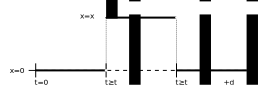
\includegraphics{figures/event}
\par
\end{centering}
\caption{A singular event}
\end{figure}

### Event-based pacing systems

A system is an ordered sequence of events.
It defines a pacing value $p$ and a special event, called the
 \emph{current event} that determines $p$'s value.
If there is no current event $p=0$.

Rules:

\begin{itemize}
\item No two events in a pacing system may start or re-occur at the same time.
\item Whenever an event $i$ starts, it becomes the current event and the pacing
 variable's value changes to $p=p_i$.
\item When a second event $j$ starts during, or just after the current event,
 it becomes the current event and $p=p_j$.
\item When the current event deactivates, $p$ becomes zero, regardless of any
 previous events that may still be active.
\end{itemize}

Three examples of special cases are shown in \fig{pacing-examples}.

\begin{figure}
\noindent
\begin{centering}
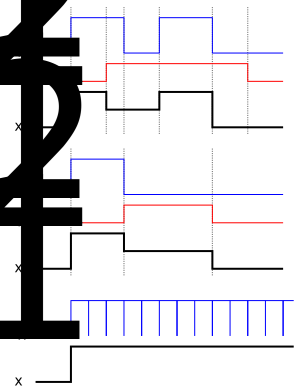
\includegraphics{figures/pacing-examples}
\par
\end{centering}
\caption{
\label{fig:pacing-examples}
Three examples of pacing:
\textit{(Top)} Three overlapping events
\textit{(Middle)} Event 1 deactivates just when event 2 activates, the pacing
 level never goes down to zero but jumps from $p_1$ to $p_2$.
\textit{(Bottom)} An indefinitely re-occuring event with $d_i = r_i$: the pacing
 value stays at $p_i$ without interruption.
}
\end{figure}

### Why event-based pacing

The two most common pacing methods used in cardiac cell simulation are (1) a
 periodic brief block current, or stimulus, and (2) a series of voltage steps.
Both cases fit neatly into the event-based scheme.

These protocols could also be implemented as part of the model\footnote{
 Conceptually, they are outside the cell and therefore outside the model.
 But then again, so are the physical constants and external concentrations
  frequently included in cell models.
  }
However, a typical stimulus current is a 0.5ms pulse given once every 1000ms.
For an efficient, variable step-size solver, this means there is a very large
 chance the solver will step over the stimulus completely.
A simple way to remedy this is to limit the maximum step size to <0.5ms, but
 (1) this requires the solver to know about the protocol and (2) this ruins the
 efficiency of the variable step-size scheme, especially in the diastolic
 phases, where step sizes can easily exceed 100ms.
A much better way to fix it is to tell the solver where the discontinuities
 are, so that it can ensure it doesn't step over them.
This is what the event-based protocol achieves.

## Fixed-form pacing

In real experiments, an "AP-clamp" or "data-clamp" protocol is sometimes
 employed during which a pre-calculated time-series signal is applied to the
 cell, either as a current or a voltage \citep{Bebarova2012PatchClamp}.
In Myokit single-cell simulations, there are two several ways to achieve
 something similar:

\begin{enumerate}
\item For piecewise constant signals, use the event-based pacing protocol. This
 is the most efficient method.
\item For sinusoidal or other time-dependent, continuous signals, add equations
 to the model.
\item For signals with a piecewise constant part and a more complicated part,
 split the simulation into two or more parts
\item If there is no other option, use the \emph{fixed-form pacing}
 capabilities of the \code{Simulation} class.
 \end{enumerate}

Fixed-form pacing allows you to specify a time series as a tuple
 \code{(times, values)} where \code{times} is a list of $n_{points}$ times and
 \code{values} is the corresponding list of $n_{points}$ pacing values.
The times array may contain duplicates, but must be strictly non-decreasing.
For any time $t$, the value of the pacing variable is then defined by:

\begin{itemize}
\item Searching for indices $i$ and $i+1$ such that $t_i <\leq t < t_{i+1}$.
\item If such an interval can be found, the value is calculated from values
 $v_i$ and $v_{i+1}$ using linear interpolation.
\item If the requested time is earlier than the first time, the first value is
 used.
\item If the requested time is later than the last time, the last value is
 used.
\end{itemize}

Using bisection search, this can be implemented quickly.
However, (1) the interpolation is still only an approximation of the `true'
 value of whatever process generated the time series.
And (2), the interpolated function is not smooth: its derivatives have
 discontinuities at all points $(t_i, v_i)$.

## No pacing

The absence of a pacing protocol (event-based \emph{or} fixed-form) is treated
 as \emph{an empty event-based protocol}.
As a result, during a simulation without a protocol, the pacing variable and
 any variable bound to it will have value $0$.

An alternative idea was to have the pacing variable be undefined if there was
 no protocol.
In this case, any variables bound to the pacing variable would become unbound
 and would retain its original, user-specified value.
\emph{However}, this would allow variables to change from bound to unbound
 without (A) changes to the model or (B) a change in simulation engine.
So by removing a protocol the result of running a simulation with
 \code{log=myokit.BOUND} would change.
In addition, the documentation would become a great deal more complicated.
\emph{Decision:} Simulations without a protocol set the pacing variable to
 zero.

